\documentclass[tikz,border=2pt]{standalone}
\usepackage{amsmath,amssymb}
\usepackage{xcolor}
\usetikzlibrary{positioning}
\begin{document}
% Extracted from namuenofull.inc; source column: \footnotesize \cite{NU}$_{\rm p{ 175 }}$ I$^*_{n}$-IV$^*$-$\alpha$
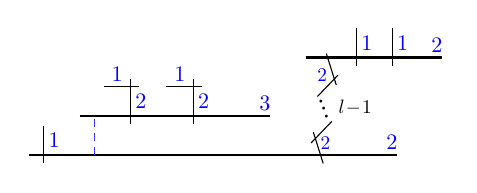
\begin{tikzpicture}[xscale=0.57,yscale=0.62]
\draw[thick,shorten >=2] (-1/3,0)--(8,0) node[inner sep=2pt,blue,above left,scale=0.8] {2} node[inner sep=2pt,below left,scale=0.8] {};
\draw[shorten <=-3pt] (0,0)--node[inner sep=2pt,scale=0.8,blue,right] {1} (0,3/5);
\draw[blue!80!white,densely dashed] (17/15,0)--(17/15,4/5);\draw[thick,shorten >=2] (4/5,4/5)--(31/6,4/5) node[inner sep=2pt,blue,above left,scale=0.8] {3} node[inner sep=2pt,below left,scale=0.8] {};
\draw[shorten <=-3pt, shorten >=-3pt] (29/15,4/5)--node[inner sep=2pt,scale=0.8,blue,right] {2} (29/15,7/5);
\draw[shorten <=-3pt] (29/15,7/5)--node[inner sep=2pt,scale=0.8,blue,above] {1} (4/3,7/5);
\draw[shorten <=-3pt, shorten >=-3pt] (10/3,4/5)--node[inner sep=2pt,scale=0.8,blue,right] {2} (10/3,7/5);
\draw[shorten <=-3pt] (10/3,7/5)--node[inner sep=2pt,scale=0.8,blue,above] {1} (41/15,7/5);
\draw (37/6,0) 
    ++(0.06,-0.17)--++(-0.22,0.64)++(0.11,-0.24)  
    ++(0,0.02)
      node[blue,scale=0.7,inner sep=1,anchor=west]{2}
    ++(0,-0.02)
    ++(-0.16,0.02)--++(0.46,0.44)++(-0.12,0.08)  
    node{$\cdot$} ++(-0.06,0.16) node{$\cdot$}
    ++(-0.06,0.16) node{$\cdot$}++(0.17,-0.12)    node[auto,inner sep=5,scale=0.7,anchor=west]{$l\!-\!1$}
    ++(-0.25,0.23)--++(0.46,0.44)++(-0.19,0.04)   
    ++(0,-0.05)
      node[blue,scale=0.7,inner sep=1,anchor=east]{2}
    ++(0,0.05)
    ++(0.19,-0.04)++(-0.04,-0.2)--++(-0.22,0.64);
\draw[thick,shorten >=2] (35/6,2)--(9,2) node[inner sep=2pt,blue,above left,scale=0.8] {2};
\draw[shorten <=-3pt] (209/30,2)--node[inner sep=2pt,scale=0.8,blue,right] {1} (209/30,13/5);
\draw[shorten <=-3pt] (233/30,2)--node[inner sep=2pt,scale=0.8,blue,right] {1} (233/30,13/5);
\end{tikzpicture}
\end{document}
